\documentclass[12pt]{article}
\usepackage{tikz}
\usepackage{geometry}

\usetikzlibrary{mindmap}

\author{ supercentinel }
%2019-01-01
\geometry{landscape, margin=1cm}

\begin{document}
\begin{center}
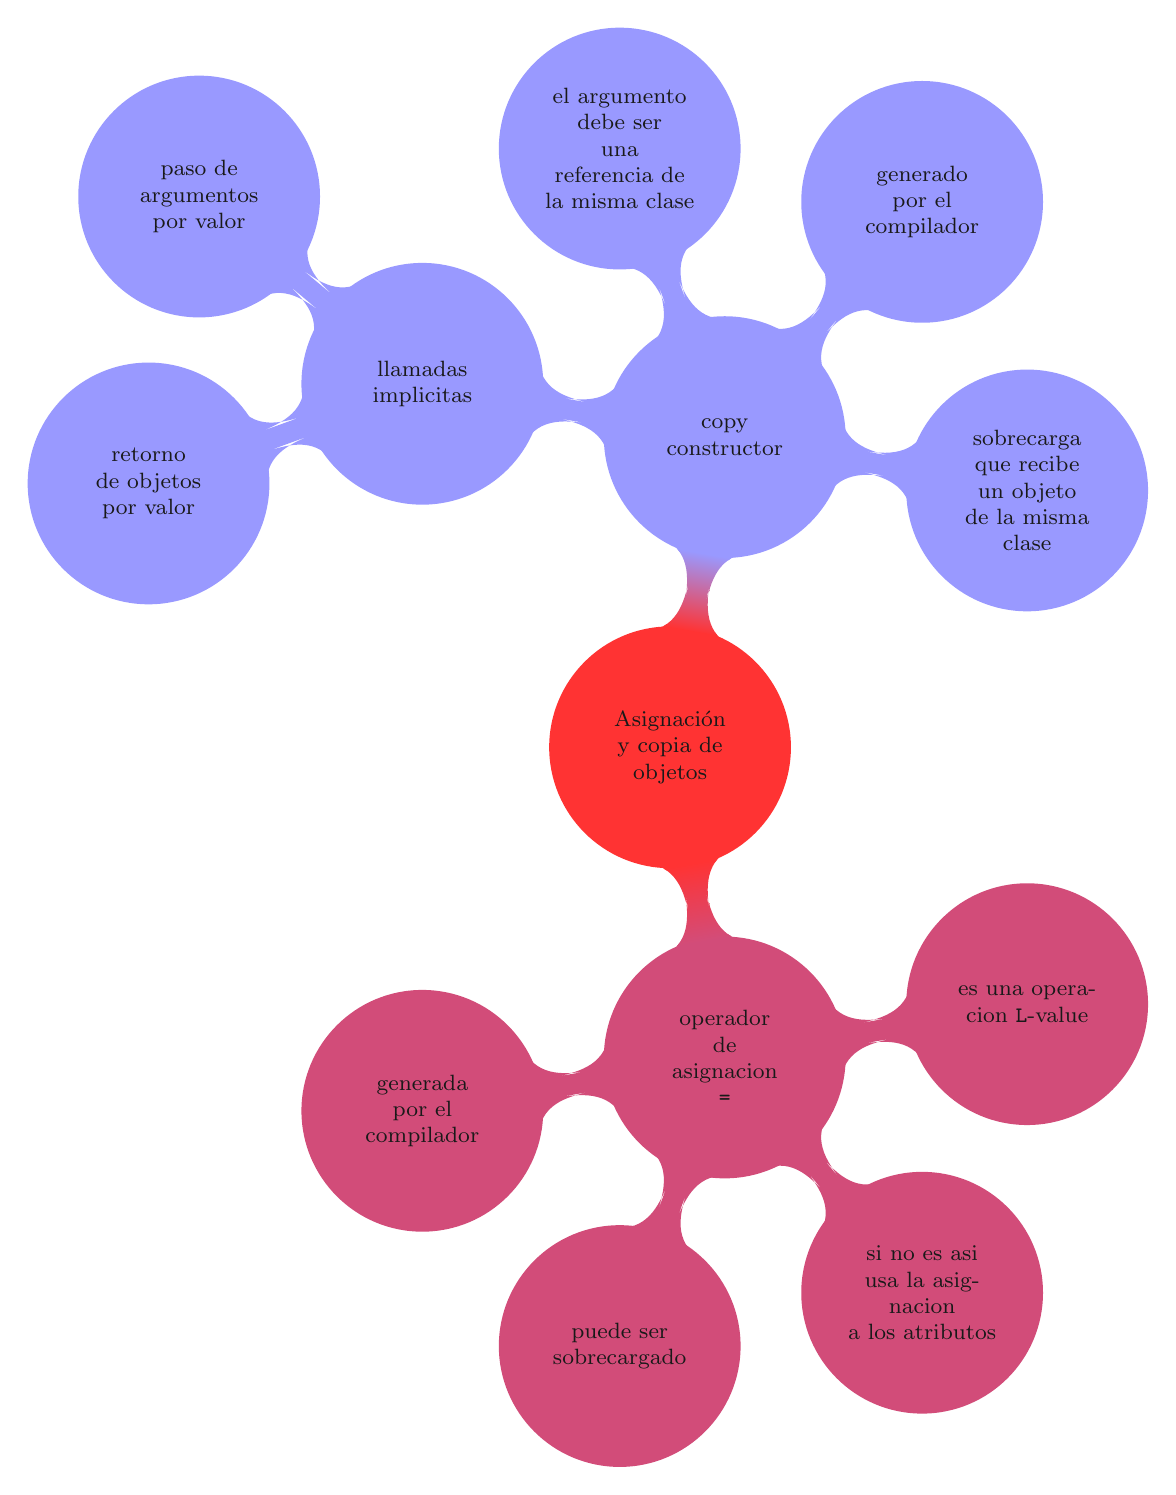
\begin{tikzpicture}[small mindmap, grow cyclic, every node/.style=concept, concept color=red!80, text=black!90, minimum size=3.0cm,
    level 1/.style={level distance=4.5cm,sibling angle=360/4},
    level 1/.style={level distance=4.0cm,sibling angle=160},
    level 2/.style={level distance=3.9cm,sibling angle=60},
    level 3/.style={level distance=3.7cm,sibling angle=60},
    ]
    \node{ Asignación y copia de objetos }
    child[concept color=purple!70] { node { operador\\de\\asignacion\\\texttt{=} }
        child { node { generada\\por el\\compilador } }
        child { node { puede ser sobrecargado } }
        child { node { si no es asi\\usa la asignacion\\a los atributos } }
        child { node { es una operacion \texttt{L}-value } }
    }
    child[concept color=blue!40] { node { copy\\constructor }
        child { node { sobrecarga\\que recibe\\un objeto\\de la misma\\clase } }
        child { node { generado\\por el\\compilador } }
        child { node { el argumento\\ debe ser\\una\\referencia de la misma clase } }
        child { node { llamadas implicitas }
            child { node { paso de argumentos\\por valor } }
            child { node { retorno de objetos\\por valor } }
        }
    }
    ;
\end{tikzpicture}
\end{center}
\end{document}
